%!TEX root = ../research_proposal.tex

In order to classify the research on the different fields related to software maintenance, we can reason about types of bugs at different levels. For
example, we can group bugs based on the developers that fix
them or using information about the bugs such as crash traces.


Our aim is not to improve testing as it is the case in the work of Eldh \cite{Eldh2001} and Hamill et al.\cite{Hamill2014}.
Our objective is to propose a classification that can allow researchers in the filed of mining bug 9 repositiories to use the taxonomy as a new criterion in triaging, prediction, and reproduction of bugs.
By analogy, we can look at the proposed bug taxonomy in a similar way as the clone taxonomy presented by Kapser and Godfrey \cite{CoryKapser}.
The authors proposed seven types of source code clones and then conducted a case study, using their classification, on the file system module of the Linux operating system.
This clone taxonomy continues to be used by researchers to build better approaches for detecting a given clone type and being able to effectively compare approaches with each other.

In this section, we are interested in bugs that share similar fixes.
By a fix, we mean a modification (adding or deleting lines of
code) to an exiting file that is used to solve the bug. With this
in mind, the relationship between bugs and fixes can be
modeled using the UML diagram in Figure \ref{fig:bug-taxo-diag}. The diagram
only includes bugs that are fixed. From this figure, we can
think of four instances of this diagram, which we refer to as
bug taxonomy or simply bug types (see Figure \ref{fig:bug-taxo}).



\begin{figure}[h!]
  \centering
    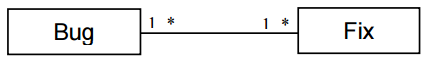
\includegraphics[scale=0.5]{media/bug-taxo-class-diag.png}
    \caption{Class diagram showing the relationship between bugs and fixed
    \label{fig:bug-taxo-diag}}
\end{figure}

\begin{figure}[h!]
  \centering
    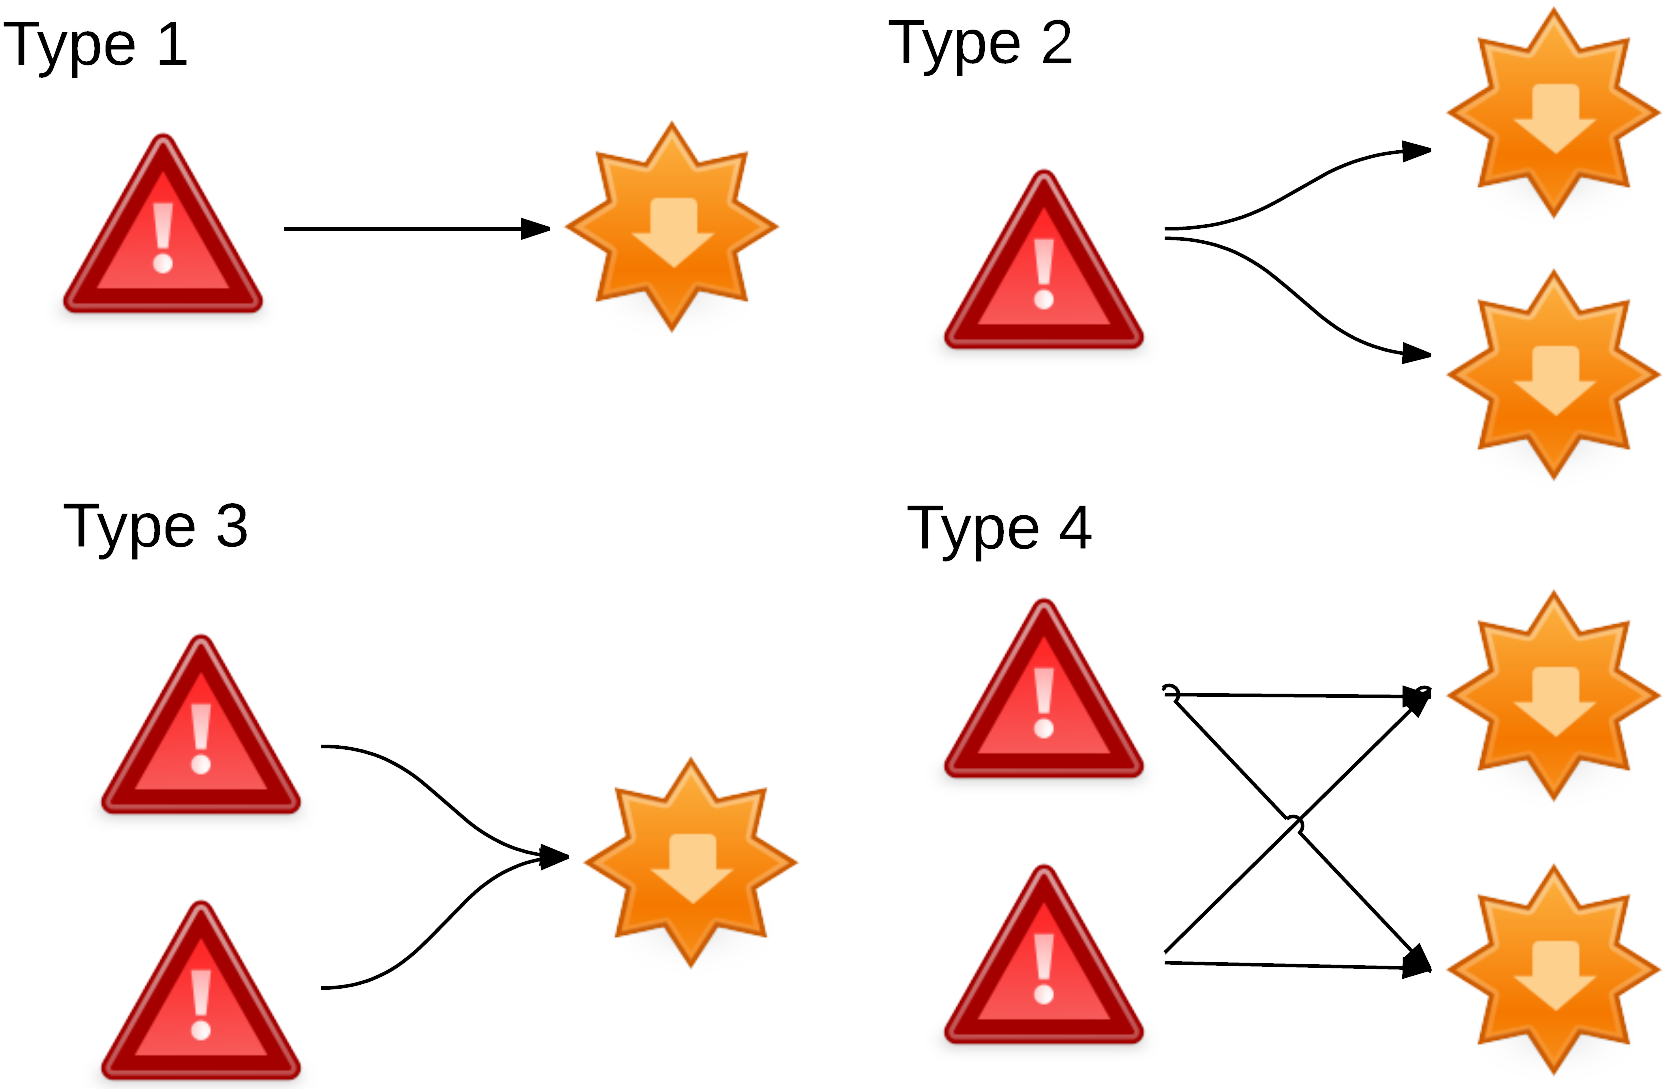
\includegraphics[scale=0.8]{media/bug-taxo.png}
    \caption{Proposed Taxonomy of Bugs
    \label{fig:bug-taxo}}
\end{figure}


The first and second types are the ones we intuitively know
about. Type 1 refers to a bug being fixed in one single location
(i.e., one file), while Type 2 refers to bugs being fixed in more
than one location. In Figure 2, only two locations are shown
for the sake of clarity, but many more locations could be
involved in the fix of a bug. Type 3 refers to multiple bugs that
are fixed in the exact same location. Type 4 is an extension of
Type 3, where multiple bugs are resolved by modifying the
same set of locations. Note that Type 3 and Type 4 bugs are
not duplicates, they may occur when different features of the
system fail due to the same root causes (faults).
We conjecture that knowing the proportions of each type
of bugs in a system may provide insight into the quality of the
system. Knowing, for example, that in a given system the
proportion of Type 2 and 4 bugs is high may be an indication
of poor system quality since many fixes are needed to address
these bugs. In addition, the existence of a high number of
Types 3 and 4 bugs calls for techniques that can effectively
find bug reports related to an incoming bug during triaging.
This is similar to the many studies that exist on detection of
duplicates (e.g., \cite{Runeson2007,Sun2010,Nguyen2012}), except that we are not looking for
duplicates but for related bugs (bugs that are due to failures of
different features of the system, caused by the same faults). To
our knowledge, there is no study that exmpirically examines
bug data with these types in mind, which is the main objective
of this section. More particularly, we are interested in the
following research questions:

\begin{itemize}
	\item RQ1: What are the proportions of different types of bugs?
	\item RQ2: How complex is each type of bugs?
	\item RQ3: How fast are these types of bugs fixed?
\end{itemize}


\section{Study Setup}

Figure \ref{fig:bug-taxo-flow} illustrates our data collection and analysis
process that we present here and discuss in more detail in the
following subsections. First, we extract the raw data from the
two bug report management systems used in this study
(Bugzilla and Jira). Second, we extract the fix to the bugs
from the source code version control system of Netbeans and
Apache (Maven and Git).

\begin{figure}[h!]
  \centering
    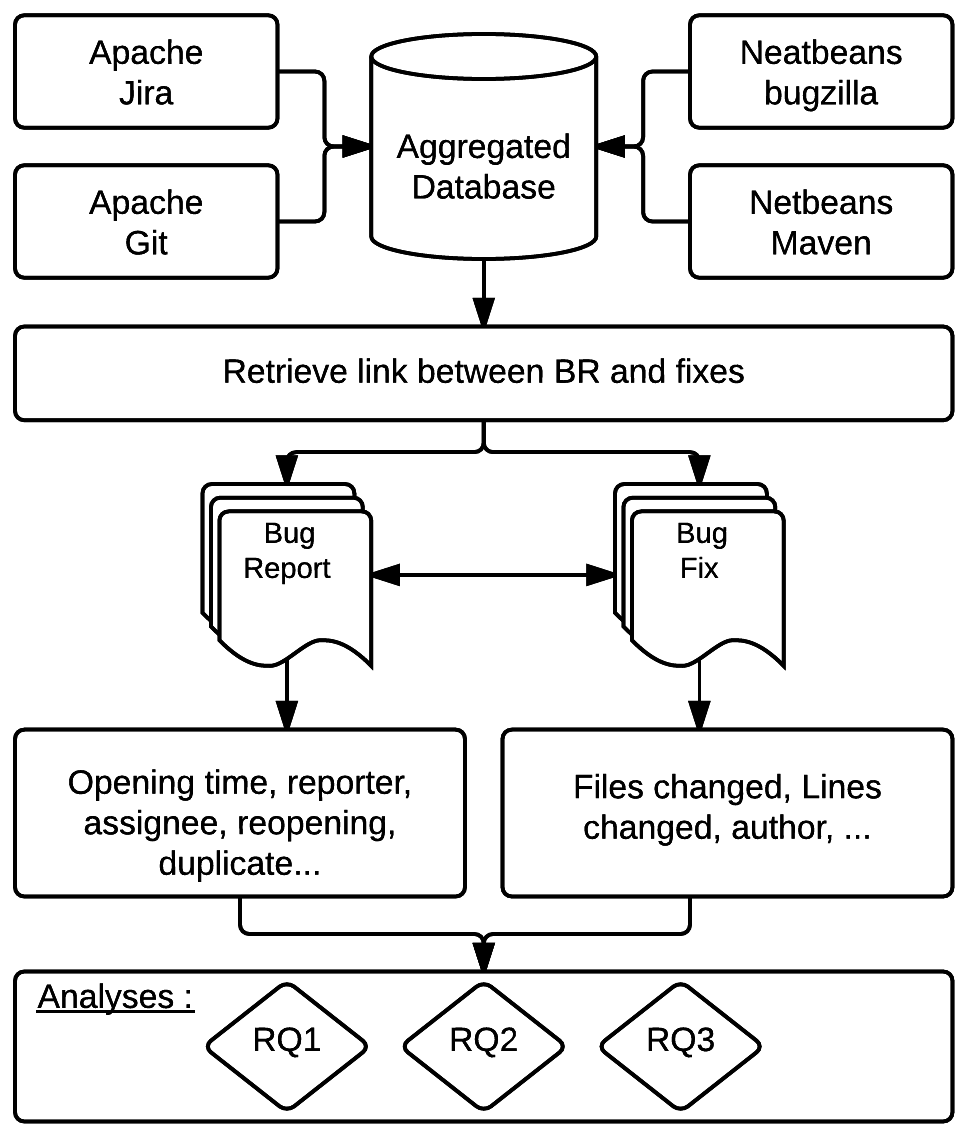
\includegraphics{media/bug-taxo-flow.png}
    \caption{Data collection and analysis process of the study
    \label{fig:bug-taxo-flow}}
\end{figure}


The extracted data is
consolidated in one database where we associate each bug
report to its fix. We mine relevant characteristics of BRs and
their fixes such as opening time, number of comments,
number of times the BR is reopened, number of changesets
for BR and the number of files changed and lines modified
for fixes or patch. Finally, we analyze these characteristics to
answer the aforementioned research questions (RQ).


\section{Datasets}

In this study, we used two distinct datasets: Netbeans and
the Apache Software Foundation projects. Netbeans is an
integrated development environment (IDE) for developing
with many languages including Java, PHP, and C/C++. The
very first version of Netbeans, then known as Xelfi, appeared
in 1996. The Apache Software Foundation is a U.S non-profit
organization supporting Apache software projects such as the
popular Apache web server since 1999. The characteristics of
the Netbeans and Apache Software Foundation are presented in Table \ref{table:datasets}.

\begin{table}[h]
\begin{center}
\begin{tabular}{@{}c|c|c|c|c@{}}
\textbf{Dataset} & \textbf{R/F BR} & \textbf{CS} & \textbf{Files} & \textbf{Projects} \\ \hline \hline
Netbeans         & 53,258          & 122,632     & 30,595         & 39                \\
Apache           & 49,449          & 106,366     & 38,111         & 349               \\
Total            & 102,707         & 229,153     & 68,809         & 388               \\ \hline \hline

\end{tabular}
\end{center}

\caption{Datasets\label{table:datasets}}
\end{table}

Cumulatively, these datasets span from 2001 to 2014. In
summary, our consolidated dataset contains 102,707 bugs,
229,153 changesets, 68,809 files that have been modified to
fix the bugs, 462,848 comments, and 388 distinct systems.
We also collected 221 million lines of code modified to fix
the bugs, identified 3,284 sub-projects, and 17,984 unique
contributors to these bug report and source code version
management systems. Finally, the cumulated opening time for
all the bugs reaches 10,661 working years (3,891,618
working days).

\section{Study Design}

We describe the design of our study by first stating the
research questions, and then explaining the variables, and
analysis methods we used to answer these questions. We
formulate three research questions (RQs) with the ultimate
goal to improve our understanding of each bug type. We
focus, however, on Types 2 and 4. This is because these bugs
require multiple fixes. They are therefore expected to be more
complex.
The objective of the first research question is to analyze
the proportion of each type of bugs. The remaining two
questions address the complexity of the bugs and the bug
fixing duration according to the type of bugs.
1)

\subsection{RQ 1: What are the proportions of different types of bugs?}

The answer to this question provides insight into the
distribution of bugs according to their type with a focus on
Type 2 and 4 bugs. As discussed ealier, knowing, for
example, that bugs of Type 2 and 4 are the most predominant
ones suggests that we need to investigate techniques to help
detect whether an incoming bug is of Types 2 and 4 by
examining historical data. Similarly, if we can automatically
identify a bug that is related to another one that has been fixed
then we can reuse the results of reproducing the first bug in
reproducing the second one.

{\bf Hypothesis}: To answer this question, we analyze whether
Type 2 and 4 bugs are predominant in the studied systems, by
testing the null hypothesis:

\begin{itemize}
	\item $H_{01A}$ : The proportion of Types 2 and 4 does not
change significantly across the studied systems
\end{itemize}


We test this hypothesis by observing both a “global”
(across systems) and a “local” predominance (per system) of
the different types of bugs. We must observe these two
aspects to ensure that the predominance of a particular type of
bug is not circumstantial (in few given systems only) but is
also not due to some other, unknown factors (in all systems
but not in a particular system).

{\bf Variables}: We use as variables the amount of resolved/fixed
bugs of each type (1, 2, 3 and 4) that are linked to a fix
(commit). As mentioned earlier, duplicate bugs are excluded.
These are marked as resolved/duplicate in our dataset.

{\bf Analysis Method}: We answer RQ1 in two steps. The first
step is to use descriptive statistics; we compute the ratio of
Types 2 and 4 bugs and the ratio of Types 1 and 3 bugs to the
total number of bugs in the dataset. This shows the
importance of Types 2 and 4 bugs compared to Types 1 and 3
bugs.

In the second step, we compare the proportions of the
different types of bugs with respect to the system where the
bugs were found. We build the contingency table with these
two qualitative variables (the type and studied system) and
test the null hypothesis H 01A to assess whether the proportion
of a particular type of bugs is related to a specific system or
not.

We use the Pearson's chi-squared test to reject the null
hypothesis $H_{01A}$ . Pearson’s chi-squared independence test is
used to analyze the relationship between two qualitative data,
in our study the type bugs and the studied system. The results
of Pearson’s chi-squared independence test are considered
statistically significant at $\alpha$ = 0.05. If p-value $\le$ 0.05, we
reject the null hypothesis $H_{01A}$ and conclude that the
proportion of types 3 and 4 bugs is different from the
proportion of type 1 and 2 bugs for each system.

\subsection{RQ 2: How complex is each type of bugs?}

We address the relation between Types 2 and 4 bugs and
the complexity of the bugs in terms of severity, duplicate and
reopened.We analyze whether Types 2 and 4 bugs are more
complex to handle than Types 1 and 3 bugs, by testing the
null hypotheses:

\begin{itemize}
 \item  $H_{02S}$ : The severity of Types 2 and 4 bugs is not
significantly different from the severity of Types 1 and 3
 \item  $H_{02D}$ : Types 2 and 4 bugs are not significantly more
likely to get duplicated than Types 1 and 3.
 \item  $H_{02R}$ : Type 2 and 4 bugs are not significantly more
likely to get reopened than Types 1 and 3.
\end{itemize}

{\bf Variables}: We use as independent variables for the
hypotheses $H_{02S}$ , $H_{02D}$ , $H_{02R}$ the bug type (if the bug is from
Types 2 and 4 or if it is from Types 1 and 3). For $H_{02S}$  we use
the severity as dependent variable to assess the relationship
between the bug severity and the bug type. For $H_{02D}$
(respectively $H_{02R}$) we use a dummy variable duplicated
(reopened) to assess if a bug has been duplicated (reopened)
at least once or not. This will be used to assess the
relationship between the type of the bugs and the fact that the
bug is more likely to be reopened or duplicated.

{\bf Analysis Method}: For each hypothesis, we build a
contingency table with the qualitative variables type of bugs
(2 and 4 or 1and 3) and the dependent variable duplicated
(respectively reopened) and the severity variable.

We use the Pearson’s chi-squared test to reject the null
hypothesis $H_{02D}$ (respectively $H_{02R}$ ) and $H_{02S}$. The results of
Pearson’s chi-squared independence test are considered
statistically significant at $\alpha$ = 0.05. If a p-value $\le$ 0.05, we
reject the null hypothesis  $H_{02D}$ (respectively $H_{02R}$) and
conclude the fact that the bug is more likely to be duplicated
(respectively reopened) is related to the type of the bug and
we reject $H_{02S}$ and conclude that the severity level of the bug
is related to the bug type.

\subsection{RQ 3 : How fast are these types of bugs fixed ?}

In this question, we study the relation between the
different types of bugs and the fixing time. We are interested
in evaluating whether developers take more time to fix Types
2 and 4 bugs than Type 1 and 3, by testing the null hypothesis:

\begin{itemize}
	\item $H_{03}$ : There is no statistically-significant difference
between the duration of fixing periods for Types 2 and
4 bugs and that of Types 1 and 3 bugs.
\end{itemize}


{\bf Variables}: To compare the bug fixing time with respect to
their type, we use as independent variable the type Ti of a
bug Bi, to distinguish between Types 1 and 3 bugs and Types
2 and 4 bugs. We consider as dependent variable the fixing
time, FTi, of the bug Bi. We compute the fixing time FTi of a
bug Bi. The fixing time FTi is the time between when the bug
is submitted to when it is closed/fixed.

{\bf Analysis Method}: We compute the (non-parametric) Mann-
Whitney test to compare the BR fixing time with respect to
the BR type and analyze whether the difference in the average
fixing time is statistically significant. We use the Mann-
Whitney test because, as a non-parametric test, it does not
make any assumption on the underlying distributions. We
analyze the results of the test to assess the null hypothesis
$H_{03}$ . The result is considered as statistically significant at $\alpha$ =
0.05. Therefore, if p-value $\le$ 0.05, we reject the null
hypothesis H 03 and conclude that the average fixing time of
Types 1 and 3 bugs is significantly different from the average
fixing time of Types 2 and 4 bugs.

\section{Study result and discussion}

In this section, we report on the results of the analyses we
performed to answer our research questions. We then dedicate
a section to discussing the results.

\subsection{RQ 1 : What are the proportions of different types of
bugs?}

Figure \ref{fig:bug-taxo-rq1} shows the percentage of the different types of
bugs. As shown in the figure, we found that 65\% of the bugs
are from Types 2 and 4. This shows the predominance of this
type of bugs in all the studied systems. Figure 5 shows the
repartition per dataset. We can see that Netbeans and Apache
have 66\% and 64\% bugs of Type 1and 3, respectively. To
ensure that this observation is not related to a particular
system, we perform Pearson’s chi-squared test across the
studied systems. Table \ref{tab:bug-taxo-rq1} shows the contingency table for the
studied systems and the result of Pearson’s chi-squared test.
The results show that there is statistically significant
difference between the proportions of the different types of
bugs.

\begin{table}[h!]
\centering
\begin{tabular}{c|c|c|c}
{System} & {Type 1 and 3} & {Type 2 and 4} & {Pearson’s chisquared p-value}        \\  \hline \hline
Apache       & 4910               & 8626               & \multirow{2}{*}{p-value \textless 0,0001} \\ \cline{1-3}
Netbeans     & 9050               & 17586              & \\ \hline \hline
\end{tabular}
\caption{Contingency table and Pearson's chi-squared tests\label{tab:bug-taxo-rq1}}
\end{table}

\begin{figure}[h!]
  \centering
    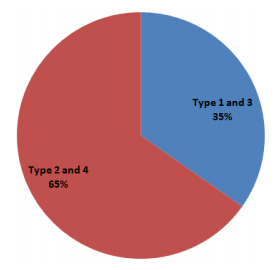
\includegraphics[scale=0.7]{media/bug-taxo-rq1.png}
    \caption{Proportions of different types of bugs
    \label{fig:bug-taxo-rq1}}
\end{figure}

Table \ref{tab:bug-taxo-rq1-prop} shows the number of bugs for each type of bugs
and the percentage of each type of bugs. We can see that
Types 3 and 4 bugs represent 28.33\% and 61.21\% of the total
of bugs, respectively. Types 1 and 2 represent only 6.78\% and
3.74\%. Together, Types 3 and 4 bugs represent almost 90\%
of the total number of bugs linked to a commit.

\begin{table}[h!]
\centering

\begin{tabular}{c|c|c|c|c|c}
Datasets                  & T1        & T2       & T3        & T4        & Total                  \\ \hline \hline
\multirow{2}{*}{Netbeans} & 776       & 240      & 8372      & 17366     & \multirow{2}{*}{26754} \\
                          & (2.90\%)  & (0.90\%) & (31.29\%) & (64.91\%) &                        \\ \hline
Apache                    & 1968      & 1248     & 3101      & 7422      & \multirow{2}{*}{13739} \\
                          & (14.32\%) & (9.08\%) & (22.57\%) & (54.02\%) &                        \\ \hline
\multirow{2}{*}{Total}    & 2744      & 1488     & 11473     & 24788     & \multirow{2}{*}{40493} \\
                          & (6.78\%)  & (3.74\%) & (28.33\%) & (61.21\%) & \\ \hline \hline
\end{tabular}
\caption{Proportion of bug types in amount and percentage}
\label{tab:bug-taxo-rq1-prop}
\end{table}


\noindent\fbox{%
    \parbox{\textwidth}{%
      We can thus reject the null hypothesis $H_{01A}$ and
conclude that there is a predominance of Types 2 and
4 bugs in all studied systems and this observation is
not related to a specific system.
    }%
}

\subsection{RQ 2 : How complex is each type of bugs?}

Figure \ref{fig:bug-taxo-rq2-prop-apache} and \ref{fig:bug-taxo-rq2-prop-netbeans} show the proportion of each bug type with
respect to their severity for each dataset. Table V shows the
proportion of each bug type with repect to their severity and
dataset. For Netbeans, the bugs we examined in our dataset
are either labeled as Blocker or Normal (despite the fact that
Netbeans uses Bugzilla that supports all the severity levels
presented in the previous section).

\begin{figure}[h!]
  \centering
    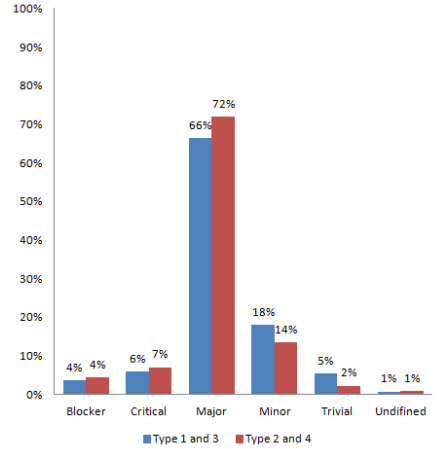
\includegraphics[scale=0.6]{media/bug-taxo-rq2-prop-apache.png}
    \caption{Proportions of Types 1 and 3 versus Types 2 and 4 with respct to their severity in the Apache dataset.
    \label{fig:bug-taxo-rq2-prop-apache}}
\end{figure}

\begin{figure}[h!]
  \centering
    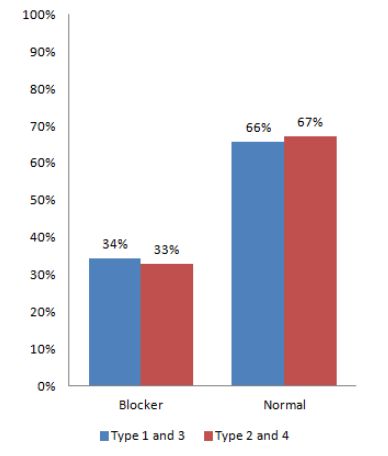
\includegraphics[scale=0.6]{media/bug-taxo-rq2-prop-netbeans.png}
    \caption{Proportions of Types 1 and 3 versus Types 2 and 4 with respct to their severity in the Netbeans dataset.
    \label{fig:bug-taxo-rq2-prop-netbeans}}
\end{figure}

For the Apache dataset, the severity levels range from
Blocker to Trivial as shown in Figure \ref{fig:bug-taxo-rq2-prop-apache}. Figure \ref{fig:bug-taxo-rq2-prop-netbeans} shows that
in Netbeans around 67\% of Types 2 and 4 bugs are normal.
The same holds for Types 1 and 3 bugs (66\% are considered
of normal severity). This indicates that most Types 2 and 4
bugs and Types 1 and 3 bugs are not critical in the Netbeans
dataset. For the Apache dataset, the results indicate that the
majority of the bugs are considered of major severity (66\%
for Types 1 and 3 and 72\% for Types 2 and 4). It is
challenging to understand the discrepancy between the two
datasets partly because of the way the severity is assigned to
BRs.

Table \ref{tab:bug-taxo-rq2-chi} shows the result of the Pearson chi-squared tests
for the $H_{02S}$, $H_{02D}$ and $H_{02R}$ hypotheses.

\begin{table}[h!]
\centering
\begin{tabular}{c|c|c}
System                    & Factor     & \begin{tabular}[c]{@{}c@{}}Pearson’s chisquared\\ p-value\end{tabular} \\ \hline \hline
\multirow{3}{*}{Apache}   & Severity   & p-value \textless 0.005                                                \\
                          & Reopened   & p-value \textless 0.005                                                \\
                          & Duplicated & p-value \textless 0.005                                                \\ \hline \hline
\multirow{3}{*}{Netbeans} & Severity   & p-value \textless 0.005                                                \\
                          & Reopened   & p-value \textless 0.005                                                \\
                          & Duplicated & p-value \textless 0.005  \\  \hline \hline
\end{tabular}

\caption{Pearson's chi squared p-values for the severity, the reopen and the duplicate factor with respect to a dataset}
\label{tab:bug-taxo-rq2-chi}
\end{table}

\noindent\fbox{%
    \parbox{\textwidth}{%
      According to the results of the test (p-value < 0.005),
we reject the null hypothesis $H_{02S}$ and conclude that
there is a significant difference between the severity of
Types 1 and 3 bugs and the severity of Types 2 and 4
bugs.
    }%
}

\begin{table}[h!]
\centering
\begin{tabular}{c|c|c|c|c}
Severity                  & T1      & T2      & T3      & T4      \\
\hline \hline
\multicolumn{5}{c}{Netbeans}                                      \\ \hline
\multirow{2}{*}{Blocker}  & 340     & 109     & 2850    & 5687    \\
                          & 43.81\% & 45.42\% & 34.04\% & 32.75\% \\ \hline
\multirow{2}{*}{Normal}   & 436     & 131     & 5522    & 11678   \\
                          & 56.19\% & 54.58\% & 65.96\% & 67.25\% \\
                          \hline
\multirow{2}{*}{Total}    & 776     & 240     & 8372    & 17365   \\
                          & 100\%   & 100\%   & 100\%   & 100\%   \\
\hline \hline
\multicolumn{5}{c}{Apache}                                        \\ \hline
\multirow{2}{*}{Blocker}  & 68      & 53      & 115     & 329     \\
                          & 3.46\%  & 4.25\%  & 3.71\%  & 4.43\%  \\
                          \hline
\multirow{2}{*}{Critical} & 84      & 44      & 213     & 565     \\
                          & 4.27\%  & 3.53\%  & 6.87\%  & 7.61\%  \\
                          \hline
\multirow{2}{*}{Major}    & 1245    & 811     & 2096    & 5427    \\
                          & 63.26\% & 64.98\% & 67.59\% & 73.12\% \\
                          \hline
\multirow{2}{*}{Minor}    & 408     & 276     & 501     & 899     \\
                          & 20.73\% & 22.12\% & 16.16\% & 12.11\% \\
                          \hline
\multirow{2}{*}{Trivial}  & 113     & 31      & 159     & 161     \\
                          & 5.74\%  & 2.48\%  & 5.13\%  & 2.17\%  \\
                          \hline
\multirow{2}{*}{Total}    & 1918    & 1215    & 3084    & 7381    \\
                          & 100\%   & 100\%   & 100\%   & 100\%  \\
\hline \hline
\end{tabular}
\caption{Proportion of each bug type with respect to severity.}
\label{tab:bug-taxo-rq2-severity}
\end{table}

Table \ref{tab:bug-taxo-rq2-dup} shows the occurrences of duplicate and reopened
bugs with respect to their bug type in each dataset. In
Netbeans, the proportion of Type 1 bugs that are marked as
source of duplicate is 6.06\%, 4.59\% for Type 2 bugs, 5.09\%
for Type 3 bugs and 5.87\% for Type 4 bugs with a total of
1503 bugs over 26754 (5.62\%). In Apache, the proportion of
Type 1 bug marked a source of a duplicate is 2.59\% and
2.24\%, 1.61\% and 2.91\% for Types 2, 3 and 4, respectively.

\begin{table}[h!]
\centering
\begin{tabular}{c|c|c|c|c|c}
Type                   & T1     & T2     & T3     & T4     & Total  \\ \hline \hline
\multicolumn{6}{c}{Netbeans}                                      \\ \hline \hline
\multirow{2}{*}{Dup.}  & 6.06\% & 4.59\% & 5.09\% & 5.87\% & 5.62\% \\
                       & (47)   & (11)   & (426)  & (1019) & (1503) \\ \hline
\multirow{2}{*}{Reop.} & 4.38\% & 7.08\% & 4.81\% & 7.09\% & 6.30\% \\
                       & (34)   & (17)   & (403)  & (1231) & (1685) \\ \hline
\multicolumn{6}{c}{Apache}                                        \\ \hline \hline
\multirow{2}{*}{Dup}   & 2.59\% & 2.24\% & 1.61\% & 2.91\% & 2.51\% \\ \
                       & (51)   & (28)   & (50)   & (216)  & (345)  \\ \hline
\multirow{2}{*}{Reop}  & 5.59\% & 6.49\% & 3.10\% & 6.90\% & 5.82\% \\
                       & (110)  & (81)   & (96)   & (512)  & (799)  \\ \hline
\multicolumn{6}{c}{Total}                                         \\ \hline \hline
\multirow{2}{*}{Dup}   & 3.57\% & 2.62\% & 4.15\% & 4.98\% & 4.56\% \\
                       & (98)   & (39)   & (476)  & (1235) & (1848) \\ \hline
\multirow{2}{*}{Reop}  & 5.25\% & 6.59\% & 4.35\% & 7.03\% & 6.13\% \\
                       & (144)  & (98)   & (499)  & (1743) & (2484) \\ \hline
\end{tabular}
\caption{Percentage and occurences of bugs duplicated by other bufs and reopenned with respect to their bug type and dataset.}
\label{tab:bug-taxo-rq2-dup}
\end{table}

Second, we analyze the reopened bugs to see the link
between the reopening and the type of bugs. We perform
Pearson’s chi-squared test to reject the null hypothesis $H_{02R}$.

\noindent\fbox{%
    \parbox{\textwidth}{%
      According to the results of the test (p-value <
0.005), we reject the null hypothesis $H_{02R}$ and
conclude that there is a significant relationship
between the reopening of a bug and its type.
    }%
}

Third, we analyze the duplicated bugs to see if there is a
link between the bug type and the fact duplication. We
perform Pearson’s chi-squared test to reject the null
hypothesis $H_{02D}$.

\noindent\fbox{%
    \parbox{\textwidth}{%
      According to the results of the test (p-value <
0.005), we reject the null hypothesis $H_{02D}$ and
conclude that there is a significant relationship
between the duplication of a bug and its type.
    }%
}

\subsection{RQ 3 : How fast are these types of bugs fixed ?}

Figure \ref{fig:bug-taxo-rq3} shows the fixing time for Types 1 and 3 versus
Types 2 and 4 for Netbeans and the Apache Software
Foundation. In Netbeans, 98.96 and 137.05 days are required
to fix Types 1 and 3 and Types 2 and 4, respectively. In
Apache, 55.76 and 85.48 days are required to fix Types 1 and
3 and Types 2 and 4, respectively.


\begin{figure}[h!]
  \centering
    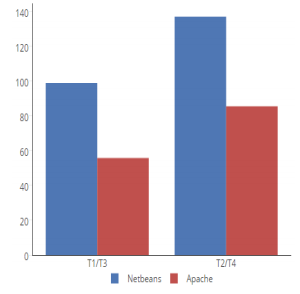
\includegraphics[scale=0.8]{media/bug-taxo-rq3.png}
    \caption{Fixing time of Types 1 and 3 versus fixing time of Types 2 and 4.
    \label{fig:bug-taxo-rq3}}
\end{figure}

Table \ref{tab:bug-taxo-rq3} shows the average fixing time of bugs with respect
to their bug type in each dataset.

\begin{table}[h!]
\centering
\begin{tabular}{c|c|c|c|c|c}
Dataset  & T1    & T2     & T3     & T4     & Average \\ \hline \hline
Netbeans & 97.66 & 117.42 & 100.26 & 156.67 & 118.00  \\ \hline
Apache   & 73.48 & 118.12 & 38.04  & 52.83  & 70.62   \\ \hline
Total    & 85.57 & 117.77 & 69.15  & 104.75 & 94.31  \\ \hline \hline
\end{tabular}
\caption{Average fixing time with respect to bug type
    \label{tab:bug-taxo-rq3}}
\end{table}

We analyze the difference in the fixing time of bugs with
respect to their bug type by conducting a Mann-Whitney test
to assess $H03$.The results show that the difference between
the fixing time of Types 2 and 4 and Types 1 and 3 is
statistically significant (p-value < 0,005).

\noindent\fbox{%
    \parbox{\textwidth}{%
      Therefore, we can reject the null hypothesis $H03$ and
conclude that the fixing of Types 2 and 4 bugs takes
more time than the fixing of Types 1 and 3 bugs.
    }%
}

\subsubsection{Dicussion}

{\bf Repartition of bug types}: One important finding of this
study is that there is significantly more Types 2 and 4 bugs
than Types 1 and 3 in all studied systems. Moreover, this
observation is not system-specific. The traditional one-bug/
one-fault way of thinking about bugs only accounts for 35\%
of the bugs. We believe that, recent triaging algorithms
\cite{Jalbert2008,Jeong2009,Khomh2011a,Tamrawi2011a} can benefit from these findings by developing
techniques that can detect Type 2 and 4 bugs. This would
result in better performance in terms of reducing the cost,
time and efforts required by the developers in the bug fixing
process.

{\bf Severity of bugs}: We discussed the severity and the
complexity of a bug in terms of its likelihood to be reopened
or marked as duplicate (RQ2). Although clear guidelines exist
on how to assign the severity of a bug, it remains a manual
process done by the bug reporter. In addition, previous
studies, notably those by Khomh et al. \cite{Khomh2011a}, showed that severity is not a consistent/trustworthy characteristic of a BR,
which lead to he emergence of studies for predicting the
severity of bugs (e.g., \cite{Lamkanfi2010,Lamkanfi2011,Tian2012}). Nevertheless, we
discovered that there is a significant difference between the
severities of Types 1 and 3 compared to Types 2 and 4.

{\bf Complexity of bugs}: At the complexity level, we use the
number of times a bug is reopened as a measure of
complexity. Indeed, if a developer is confident enough in
his/her fix to close the bug and that the bug gets reopened it
means that the developer missed some dependencies of the
said bug or did not foresee the consequences of the fix.
We found that there is a significant relationship between
the number of reopenings and type of a bug. In other words,
there is a significant relationship between the complexity and
the type of a given bug. In our datasets, Types 1 and 3 bugs
are reopened in 1.88\% of the cases, while Types 2 and 4 are
reopened in 5.73\%. Assuming that the reopening is a
representative metric for the complexity of bug, Types 2 and
4 are three times more complex than Types 1 and 3. Finally, if
we consider multiple reopenings, Types 2 and 4 account for
almost 80\% of the bugs that reopened more than once and
more than 96\% of the bug opened more than twice.
While current approaches aiming to predict which bug
will be reopen use the amount of modified files \cite{Shihab2010,Zimmermann2012,Lo2013}, we
believe that they can be improved by taking into account the type of a the bug. For example, if we can detect that an
incoming bug if of Type 2 or 4 then it is more likely to
reopened than a bug of Type 1 or 3. Similarly, approaches
aiming to predict the files in which a given bug should be
fixed could be categorized and improved by knowking the
bug type in advance \cite{Zhou2012,Kim2013a}.

{\bf Impact of a bug}: To measure the impact of bugs in end-users
and developers, we use the number of times a bug is
duplicated. This is because if a bug has many duplicates, it
means that a large number of users have experienced and a
large number of developers are blocked the failure.
We found that there is a significant relationship between
the bug type and the fact that it gets duplicated. Types 1 and 3
bugs are duplicated in 1.41\% of the cases while Types 2 and 4
are duplicated in 3.14\%. Assuming that the amount of
duplication is an accurate metric for the impact of bug, Types
2 and 4 have more than two times bigger impact than Types 1
and 3. Similarly to reopening, if we consider multiple
duplication, Types 2 and 4 account for 75\% of the bugs that
get duplicated more than once and more than 80\% of the bugs
that get duplicated more than twice.
We believe that approaches targeting the identification of
duplicates \cite{Bettenburg2008a,Jalbert2008,Sun2010,Tian2012a}  could leverage this taxonomy to
achieve even better performances in terms of recall and
precision.

{\bf Fixing time}: Our third research question aimed to determine
if the type of a bug impacts its fixing time. Not only we found
that the type of a bug does significantly impact its fixing time,
but we also found that, in average Types 2 and 4, stay open
111.26 days while Types 1 and 3 last for 77.36 days. Types 2
and 4 are 1.4 time longer to fix than Types 1 and 3.We
therefore believe that, approaches aiming to predict the fixing
time of a bug (e.g., \cite{Panjer2007,Bhattacharya2011,Zhang2013}) can highly benefit from
accurately predicting the type of a bug and thereforebetter
plan the required man-power to fix the bug.
In summary, Types 2 and 4 account for 65\% of the bugs
and they are more complex, have a bigger impact and take
longer to be fixed than Types 1 and 3 while being equivalent
in terms of severity.

Our taxonomy aimed to analyse: (1) the
proportion of each type of bugs; (2) the complexity of each
type in terms of severity, reopening and duplication; (3) the
required time to fix a bug depending on its type. The key
findings are:
\begin{itemize}
  \item Types 2 and 4 account for 65\% of the bugs.
  \item Types 2 and 4 have a similar severity compared to
Types 1 and 3.
  \item Types 2 and 4 are more complex (reopening) and have
a bigger impact (duplicate) than Types 1 and 3.
  \item It takes more time to fix Types 2 and 4 than Types 1
and 3.
\end{itemize}

Our taxonomy and results can be built upon in order to classify
past and new researches in several active areas such as bug
reproduction and triaging, prediction of reopening,
duplication, severity, files to fix and fixing time. Moreover, if
one could predict the type of a bug at submission time, all
these areas could be improved.
